\documentclass[10pt]{article}
\usepackage[top = 2.5cm, bottom = 2.5cm, left = 2.5cm, right = 2.5cm]{geometry} 
\usepackage[minimal=false]{../structure}

\title{Georgia Institute of Technology - Graduate Student Algebra Seminar}
\author{Connor Haynes}
\date{}

\begin{document}
\maketitle
What follows are my notes from the Graduate Student Algebra Seminar. These are not complete with respect to the original seminar, and contain additional content from my own research.
\section{Noah - Chip Firing and Census of Special Divisors}
We wish to answer two questions in this seminar:
\begin{enumerate}
\item How and why do tableaux appear when we think about chip firing games on graphs?
\item How can we prove classical results by examining problems in a tropical setting?
\end{enumerate}

First we must discuss what ``chip firing'' is. Let $G$ be a finite, loop-free graph that may or may not have parallel edges. In some contexts we may allow $G$ to be a metric graph, but this case will not be discussed in any depth here.

\begin{boxDef}{Divisor of a Graph}
  A \emph{divisor} of $G$ is a formal sum of vertices in $V(G)$ with coefficients in $\mathbb{Z}$. Any divisor $D$ takes the form
  \[D=\sum_{v\in V(G)}c_vv\]
  for some $c_V\in\mathbb{Z}$. These form a group under addition, which we denote
  \[\text{Div}(G)=\mathbb{Z}[V(G)].\]
  The \emph{degree} of a divisor $D\in\text{Div}(G)$ is given by $\text{deg}(D)=\sum_{v\in V(G)}c_v$.
\end{boxDef}

\begin{wrapfigure}{l}{0pt}
  \begin{boxNote}[width=5cm]{}
  Traditionally, chip firing games are defined such that you may only fire vertices satisfying
  \[n\geq\text{deg}(v),\]
  where $n$ is the number of chips on $v$.\\

  In this formulation,
  \[\text{Div}(G)=\mathbb{N}[V(G)].\]
  \end{boxNote}
\end{wrapfigure}

For $D\in\text{Div}(G)$, we say that a vertex $v\in V(G)$ has $n$ ``chips'' lying on it if $c_v=n$. Chip firing games are games in which players take turns ``firing'' vertices on a graph with divisor $D$.\\

To ``fire'' a vertex $v\in V(G)$ we send a single chip along each edge incident to $v$, adding $1$ to each adjacent vertex's number of chips and subtracting $\text{deg}(v)$ from the number of chips on $v$. We may wish to fire several vertices simultaneously, in which case we have that

\begin{center}
  \emph{If we choose to fire many vertices at once, chip totals change only on those vertices not in the fired set.}
\end{center}

For any two divisors $D_1$ and $D_2$ on $G$ we say that $D_1$ and $D_2$ are \emph{linearly equivalent} if one can be reached from the other by a sequence of chip firings. This defines an equivalence relation $\sim$ on $\text{Div}(G)$.

\clearpage

\begin{boxEx}{}
  Let $D_1$ and $D_2$ be the two divisors on $G$ given below. These two divisors are linearly equivalent, as $D_2$ is given by firing the bottom-left vertex of  $D_1$.

  \begin{center}
    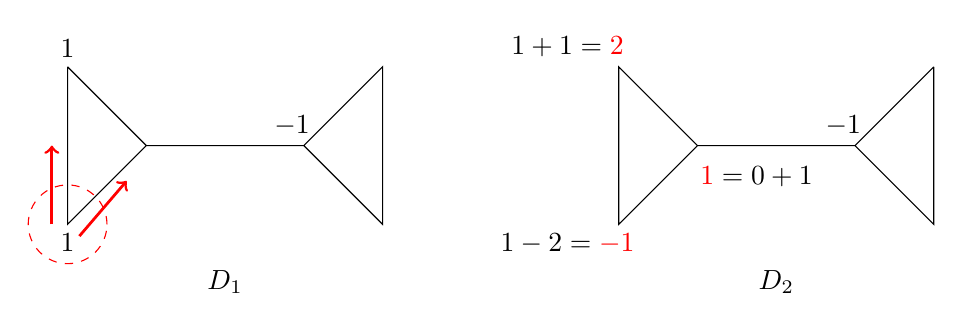
\begin{tikzpicture}
      \node [above] at (-3,-2) {$D_1$};
      \draw (-5,1) -- (-5,-1) -- (-4,0) -- (-5,1);
      \draw (-4,0) -- (-2,0) -- (-1,-1) -- (-1,1) -- (-2,0);
      \node [above] at (-5,1) {$1$};
      \node [below] at (-5,-1) {$1$};
      \node [above] at (-2.15,0) {$-1$};

      \draw [dashed, color=red] (-5,-1) circle [radius=0.5];
      \draw [->, color=red, line width=1pt] (-5.2,-1) -- (-5.2,-0);
      \draw [->, color=red, line width=1pt] (-4.85,-1.15) -- (-4.25,-0.45);
      
      \node [above] at (4,-2) {$D_2$};
      \draw (6,1) -- (6,-1) -- (5,0) -- (6,1);
      \draw (5,0) -- (3,0) -- (2,-1) -- (2,1) -- (3,0);
      \node [above] at (1.35,1) {$1+1={\color{red}2}$};
      \node [below] at (1.35,-1) {$1-2={\color{red}-1}$};
      \node [above] at (4.85,0) {$-1$};
      \node [below] at (3.75,-0.15) {${\color{red}1}=0+1$};
    \end{tikzpicture}
  \end{center}
\end{boxEx}

This equivalence relation allows us to define the Picard Group of $G$, $\text{Pic}(G)\cong\text{Div}(G)/\sim$. For the reader familiar with algebraic geometry, this seems analogous to the classical Picard Group defined over ringed spaces.\\

Hereafter when we speak of a divisor $D$ we implicity refer to its \emph{divisor class}, $[D]\in\text{Div}(G)/\sim$.

\begin{boxDef}{Rank / Canonical Divisor}
  Let $D\in\text{Div}(G)$ be a divisor. We say that $D$ is \emph{effective} if for any $v\in V(G)$, $c_V\geq0$ and write that $D\geq0$. The \emph{rank} of $D$ is given by

  \[r(D)=\begin{cases}-1 & \text{if }D\not\sim E\geq0, \\ \geq r & \text{if }\forall E\geq0 \text{ of } \text{deg}(E)=r\text{ we have }(D-E)\sim E'\geq0.\end{cases}\]

  For any graph $G$ we define the \emph{canonical divisor} to be the divisor of the form

  \[K_G=\sum_{v\in V(G)}(\text{deg}(v)-2)v.\]

  The rank of the canonical divisor is $r(K_G)=g-1$, where $g$ is the genus of $G$.
\end{boxDef}

The rank of a divisor tells us, in layman's terms, how many chips we may remove from $D$ without losing its congruence to an effective divisor. In \hyperlink{}{Example 1.3} we have that $r(D_1)=1$.\\

We are now prepared for our first major result in the study of these divisors.

\begin{boxThm}{The Riemann-Roch Theorem for Graphs\hfill Baker / Norine}
  Let $G$ be a graph and $D$ a divisor on $G$. Then
  \[r(D)=d-g+(1+r(K_G-D)).\]
\end{boxThm}
\end{document}
